\documentclass[twoside,11pt]{article}
\usepackage[left=1in, right=1in, top=1in, bottom=1in]{geometry}
\usepackage{amsmath}
\usepackage{amssymb}
\usepackage{amsfonts}
\usepackage{mathtools}
\usepackage{amsthm}
\usepackage{fancyhdr}
\usepackage{enumitem}
\usepackage{siunitx}
\usepackage{booktabs}
\usepackage[hidelinks]{hyperref}
\usepackage{sectsty}
\usepackage{mathrsfs} % mathscr
\usepackage{tikz}
\usepackage{pgfplots}
\usepackage{multicol}
\usepackage{listings}
% \usepackage{amsart}

% change mathcal shape
\usepackage[mathcal]{eucal}

% allow H option of figure
\usepackage{float}

% define math operators
\newcommand{\F}{\mathbb{F}}
\newcommand{\R}{\mathbb{R}}
\newcommand{\N}{\mathbb{N}}
\newcommand{\Z}{\mathbb{Z}}
\newcommand{\Q}{\mathbb{Q}}
\newcommand{\X}{\mathbb{Y}}
\renewcommand{\L}{\mathcal{L}}
% \renewcommand{\d}{\mathrm{d}}
\renewcommand*\d{\mathop{}\!\mathrm{d}}
\DeclareMathOperator*{\argmax}{arg\,max}
\DeclareMathOperator*{\argmin}{arg\,min}
\DeclareMathOperator{\im}{im}
\DeclareMathOperator{\id}{id}
\renewcommand{\mod}[1]{\ (\mathrm{mod}\ #1)}

% section font style
\sectionfont{\sffamily\Large}
\subsectionfont{\sffamily\normalsize}
\subsubsectionfont{\bf}

% line spreading and break
\hyphenpenalty=5000
\tolerance=20
\setlength{\parindent}{0em}
\setlength\parskip{0.5em}
\allowdisplaybreaks
\linespread{0.9}

% theorem
% latex theorem
% definition style
\theoremstyle{definition}
\newtheorem{theorem}{Theorem}[subsection]
\newtheorem{axiom}{Axiom}[section]
\newtheorem{definition}{Definition}[section]
\newtheorem{example}{Example}[section]
\newtheorem{question}{Question}[section]
\newtheorem{exercise}{Exercise}[section]
\newtheorem*{exercise*}{Exercise}
\newtheorem{lemma}{Lemma}[section]
\newtheorem{proposition}{Proposition}[section]
\newtheorem{corollary}{Corollary}[section]
\newtheorem*{theorem*}{Theorem}
\newtheorem{problem}{Problem}
% remark style
\theoremstyle{remark}
\newtheorem*{remark}{Remark}
\newtheorem*{solution}{Solution}
\newtheorem*{claim}{Claim}


% paragraph indent
\setlength{\parindent}{0em}
\setlength\parskip{0.5em}

\newcommand\Code{MAT4220 FA22}
\newcommand\Ass{HW04}
\newcommand\name{Haoran Sun}
\newcommand\mail{haoransun@link.cuhk.edu.cn}

\title{{\sffamily \Code \ \Ass}}
\author{\sffamily \name \ (\href{mailto:\mail}{\mail})}
\date{\sffamily \today}

\makeatletter
% \let\Title\@title
\let\theauthor\@author
\let\thedate\@date

\fancypagestyle{plain}{%
    \fancyhf{}
    \lhead{\sffamily \Ass}
    \rhead{\sffamily \name}
    \rfoot{\sffamily\thepage}

    % # 页脚自定义
    \fancyfoot[L]{
        \begin{minipage}[c]{0.06\textwidth}
            
\includegraphics[height=7.5mm]{logo2.png}
        \end{minipage}
    }
}
\fancypagestyle{title}{%
    \fancyhf{}
    \renewcommand{\headrulewidth}{0pt}
    % \lhead{\Title}
    % \rhead{\theauthor}
    \rfoot{\sffamily\thepage}

    % # 页脚自定义
    \fancyfoot[L]{
        \begin{minipage}[c]{0.06\textwidth}
            
\includegraphics[height=7.5mm]{logo2.png}
        \end{minipage}
    }
}
\fancyfootoffset[L]{0.3cm}

% re-define title format
\makeatletter
\renewcommand{\maketitle}{\bgroup\setlength{\parindent}{0pt}
\begin{flushleft}
  \textbf{\Large\@title}

  \@author
\end{flushleft}\egroup
}
\makeatother

\pagestyle{plain}

% lstlisting settings
\lstset{
    basicstyle=\linespread{0.7}\footnotesize,
    breaklines=true,
    basewidth=0.5em
}


\begin{document}
\maketitle
\thispagestyle{title}
% \begin{multicols*}{2}

% \begin{remark}
%     $V_\epsilon(x)$ is used to denote a $\epsilon$-neighborhood
%     \begin{align*}
%         V_\epsilon(x) = B_\epsilon(x)\setminus\{x\}
%     \end{align*}
% \end{remark}



\begin{problem}[P89 Q3]
Easy to obtain
\begin{align*}
    \frac{1}{i}\frac{T'(t)}{T(t)} &= \frac{X''(x)}{X(x)} = -\lambda
\end{align*}
and $\lambda=\beta^2\geq 0$.
Then we have
\begin{align*}
    T(t) &= e^{-i\lambda t}\\
    X(x) &= A\cos\beta x + B\sin\beta x
\end{align*}
Applying $X(0) = X(l) = 0$, we have $B=0$ and $\beta_n=n\pi/l$, $n\in\N$.
Hence
\begin{align*}
    u(x,t) &= \sum_{n=1}^\infty A_n\sin\frac{n\pi x}{l}e^{-i(n\pi)^2t/l^2}
\end{align*}
\end{problem}


\begin{problem}[P92 Q4]\
\begin{enumerate}[label=(\alph*)]
\item Easy to obtain
\begin{align*}
    \frac{1}{k}\frac{T'(t)}{T(t)} &= \frac{X''(x)}{X(x)} = -\lambda
\end{align*}
and we can show that $\lambda\geq 0$ given the periodic boundary condition.
Hence, we have $\lambda=\beta^2$ 
\begin{align*}
    X(x) &= A\cos\beta x + B\sin\beta x,\ 
    X'(x) = -A\beta\sin\beta x + B\beta\cos\beta x
\end{align*}
Plug the P.B.C into it, and we get
\begin{align*}
    X(l) &= A\cos\beta l + B\sin\beta l = X(-l) = A\cos\beta l - B\sin\beta l \\
    X'(l) &= -A\beta\sin\beta l + B\beta\cos\beta l = X'(-l) = A\beta\sin\beta l
    + B\beta\cos\beta l\\
    \Rightarrow B\sin\beta l &= A\beta\sin\beta l = 0
\end{align*}
Hence we have $\beta_n = n\pi/l$ and $\lambda_n = (n\pi/l)^2$.

\item Using the result from (a), it should be obvious that
\begin{align*}
    u(x, t) &= \frac{1}{2}A_0 + \sum_{n=1}^\infty \left(
        A_n\cos\frac{n\pi x}{l} + B_n\sin\frac{n\pi x}{l}
    \right) e^{-(n\pi/l)^2 t}
\end{align*}
\end{enumerate}
\end{problem}


\begin{problem}[P101 Q9]\
\begin{enumerate}[label=(\alph*)]
    \item Let $\lambda=0$, $X(x)=ax+b$, $X'(x)=a$.
    Plug in the boundary condition, we have
    \begin{align*}
        X_0(x) &= x - 1
    \end{align*}
    \item Let $\lambda=\beta^2$, then 
    \begin{align*}
        X(x) &= A\cos\beta x + B\sin\beta x\\
        X'(x) &= A(-\beta\sin\beta x) + B\beta\cos\beta x
    \end{align*}
    Plug in the boundary condition, we have
    \begin{align*}
        \begin{bmatrix}
            1 & \beta \\
            \cos\beta & \sin\beta
        \end{bmatrix}
        \begin{bmatrix}
            A\\B
        \end{bmatrix} &= 0
    \end{align*}
    The determinant should be zero to get non-trivial solutions
    \begin{align*}
        \sin\beta -\beta\cos\beta = 0\Rightarrow
        \tan\beta = \beta
    \end{align*}

    \item Sketch:\\
    \resizebox{0.6\textwidth}{!}{
    \def\xm{5}
    \def\ym{5}
    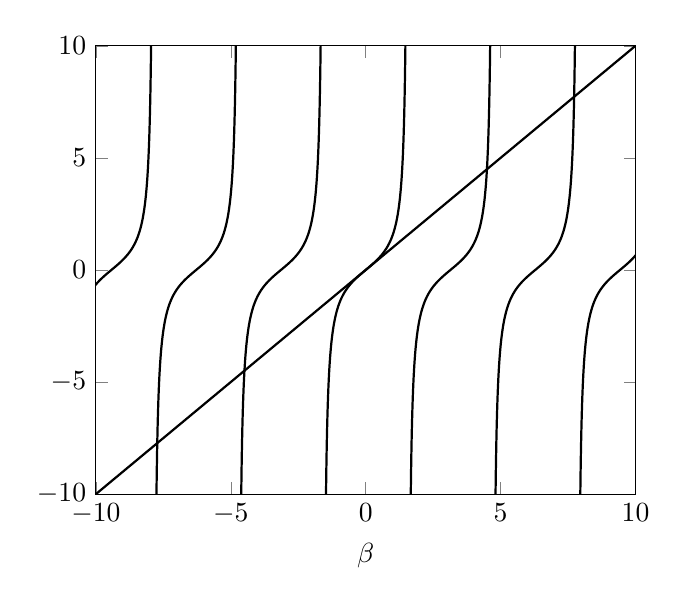
\begin{tikzpicture}
    \begin{axis}[xmax=10,xmin=-10,ymax=10,ymin=-10,xlabel=$\beta$]
        \addplot [domain=-10:10,thick,smooth,samples=200] {x};
        \foreach \i in {-5,...,5}{
            \addplot [domain=-pi/2*0.99+\i*pi:pi/2*0.99+\i*pi,thick,smooth,samples=200] {tan(deg(x};
        }
    \end{axis}
    \end{tikzpicture}
    }\\
    Thus there are infinitely many solutions.

    \item Suppose we have negative eigenvalues where $\lambda=(i\beta)^2$, then
    \begin{align*}
        X(x) &= A\cosh\beta x + B\sinh\beta x\\
        X'(x) &= A\beta\sinh\beta x + B\beta\cosh\beta x
    \end{align*}
    Since
    \begin{align*}
        X(0) &= X'(x) \Rightarrow A = B\\
        X(1) &= A\frac{e+e^{-\beta}}{2} + B\frac{e-e^{-\beta}}{2}
        = Ae^{-\beta} > 0
    \end{align*}
    thus we cannot have negative eigenvalues.
\end{enumerate}
\end{problem}


\begin{problem}[P111 Q2]\
\begin{enumerate}[label=(\alph*)]
\item For sine series
\begin{align*}
    A_n &= \frac{2}{l}\int_0^l x^2\sin\frac{n\pi}{l}\d x\\
    &=\frac{2}{n\pi}\int_0^l \left(
        \left.-x^2\cos\frac{n\pi}{l}x\right |_0^l 
        + 2\int_0^l x\cos\frac{n\pi}{l}x\d x
    \right)\\
    &= \cdots\\
    &= \left(\frac{2}{n\pi} + \frac{8}{(n\pi)^3}\right)l^2
\end{align*}
Then 
\begin{align*}
    x^2 &= \sum_{n=1}^\infty A_n n\pi x\quad\text{with}\quad
    A_n = \frac{2}{n\pi} + \frac{8}{(n\pi)^3}
\end{align*}

\item For cosine series
\begin{align*}
    A_0 &= \frac{l}{2}\int_0^l x^2\d x = \frac{2}{3}l^2\\
    A_n &= \frac{l}{2}\int_0^l x^2\cos\frac{n\pi}{l}x\d x\\
    &= \frac{2}{n\pi}\left(
        \left.x^2\sin\frac{n\pi}{l}x\right |_0^l
        -2\int_0^lx\sin\frac{n\pi}{l}x\d x
    \right)\\
    &=\cdots\\
    &= \frac{4l^2}{(n\pi)^2}
\end{align*}
Then 
\begin{align*}
    x^2 &= \frac{1}{2}A_0 + \sum_{n=1}^\infty A_n\cos\frac{n\pi}{l}x
\end{align*}
\end{enumerate}
\end{problem}


\begin{problem}[P112 Q9]
Due to the Neumann boundary condition, using the fact that
\begin{align*}
    u(x, t) &= \frac{1}{2}A_0 + \frac{1}{2}B_0 t + 
    \sum_{n=1}^n \left(
        A_n\cos\frac{n\pi}{l}t + B_n\sin\frac{n\pi c}{l}t
    \right)\cos\frac{n\pi}{l}x\\
    u(x, 0) &= \frac{1}{2}A_0 + \sum_{n=1}^n A_n\cos\frac{n\pi}{l}x = 0\\
    u_t(x, 0) &= \frac{1}{2}B_0 + \sum_{n=1}^\infty B_n\frac{n\pi c}{l}\cos\frac{n\pi}{l}x
    =\cos^2 x
\end{align*}
We can conclude that $A_n=0$ and
\begin{align*}
    B_0 &= \frac{2}{\pi}\int_0^\pi \cos^2 x\d x = 1\\
    B_n nc &= \frac{2}{\pi}\int_0^\pi \cos^2 x \cos nx\d x \\
    &= \frac{2}{\pi}\int_0^\pi \frac{1}{2}(\cos 2x + 1)\cos nx \d x\\
    &= \frac{1}{\pi}\int_0^\pi \cos 2x \cos nx + \frac{1}{\pi}\int_0^\pi\cos nx \d x\\
    &= \frac{1}{2}\delta_{2n}
\end{align*}
which means the only two non-zero terms are $B_0$ and $B_2$, therefore
\begin{align*}
    u(x,t) &= \frac{1}{2}t + \frac{1}{4c}\sin 2ct\cos 2x
\end{align*}

\end{problem}



% \end{multicols*}
\end{document}

